\documentclass[11pt,a4paper,fontset=fandol]{ctexart}

\usepackage[a4paper,margin=22mm,headheight=15pt]{geometry}
\usepackage{amsmath,amssymb}
\usepackage{graphicx}
\usepackage{booktabs,longtable,tabularx,array}
\usepackage{caption,float,pdflscape}
\usepackage{enumitem,xcolor,fancyhdr,hyperref,lastpage}
\usepackage{tikz}
\usetikzlibrary{arrows.meta,positioning,fit}

\definecolor{navy}{HTML}{17365D}
\definecolor{blue}{HTML}{2F75B5}
\definecolor{lightblue}{HTML}{DDEBF7}
\definecolor{lightgray}{HTML}{F2F2F2}
\definecolor{green}{HTML}{548235}

\hypersetup{
  colorlinks=true,
  linkcolor=navy,
  urlcolor=blue,
  pdftitle={PMSM FOC Dual Plant v2.1.0 架构与测试手册},
  pdfauthor={MatlabProgram},
  pdfsubject={FOC 双速率任务、Stateflow 电机状态机、双被控对象和自动测试结果}
}

\pagestyle{fancy}
\fancyhf{}
\fancyhead[L]{\small PMSM FOC Dual Plant v2.1.0}
\fancyhead[R]{\small 架构与测试手册}
\fancyfoot[C]{\small 第 \thepage\ 页，共 \pageref{LastPage} 页}
\renewcommand{\headrulewidth}{0.4pt}
\setlength{\parindent}{2em}
\setlength{\parskip}{0.35em}
\setlength{\emergencystretch}{2em}
\setlist[itemize]{leftmargin=2em,itemsep=0.25em,topsep=0.35em}
\setlist[enumerate]{leftmargin=2em,itemsep=0.25em,topsep=0.35em}
\captionsetup{font=small,labelfont=bf,labelsep=quad}
\renewcommand{\arraystretch}{1.22}
\setlength{\tabcolsep}{5pt}
\graphicspath{{figures/}}

\newcommand{\code}[1]{\texttt{\detokenize{#1}}}
\newcommand{\sectionline}{\vspace{-0.55em}\noindent\color{blue}\rule{\textwidth}{0.8pt}\color{black}\vspace{0.35em}}
\newcommand{\pass}{\textbf{\color{green}PASS}}

\begin{document}

\begin{titlepage}
  \centering
  \vspace*{25mm}
  {\Huge\bfseries\color{navy} PMSM FOC Dual Plant v2.1.0\par}
  \vspace{7mm}
  {\LARGE 模型架构、Stateflow 状态管理与测试手册\par}
  \vspace{15mm}
  \color{blue}\rule{0.82\textwidth}{1.2pt}\color{black}
  \vspace{14mm}

  \begin{tabular}{rl}
    \textbf{模型平台：} & MATLAB/Simulink/Stateflow R2024a \\
    \textbf{控制方案：} & 离散磁场定向控制（FOC） \\
    \textbf{被控对象：} & Native 离散 PMSM / MathWorks PMSM HDL \\
    \textbf{控制调度：} & $100\,\mu\mathrm{s}$ 电流/快速保护；1 ms 速度/状态/慢保护 \\
    \textbf{手册版本：} & v2.1.0 \\
    \textbf{验证日期：} & 2026 年 8 月 31 日 \\
  \end{tabular}

  \vfill
  {\large MatlabProgram\par}
  \vspace{8mm}
\end{titlepage}

\tableofcontents
\clearpage

\section{范围与架构依据}
\sectionline

本手册覆盖 \code{PMSM_FOC_DualPlant_v2.1.0} 模型包，说明组件化 FOC 控制器、Stateflow 电机运行状态管理、统一数据字典、类型化 Bus 接口、双 PMSM Variant 被控对象、调度边界、保护阈值、需求追溯以及自动测试结果。设计依据为项目 \path{doc/PMSM_FOC_Software_Architecture.tex} 中定义的分层控制和电机状态管理原则：数值控制算法由 Simulink 组件负责；Stateflow 只负责模式转换和监督 PWM 请求；快速保护、故障锁存和最终 PWM 仲裁由三个独立 Simulink 组件负责。

本版本控制器采用 2 个类型化 Bus 输入和 1 个 Bus 输出。输入类型为 \code{ControlCommandBus} 和 \code{MeasurementBus}；输出类型为 \code{ControlStatusBus}。

外部启动、停止、急停、驱动器故障、故障复位和硬件门控命令均已接入控制语义。标定 Bus 作为数据字典中的等价标定结构，不增加顶层零散参数线。闭环 Harness 将状态、校准、对齐和故障测试信号统一收拢到测试日志子系统。两个电机对象、平均值对象关断适配器及日志子系统仅属于仿真环境，不进入控制器 ERT 目标代码。

\subsection{主要交付文件}

\begin{itemize}[nosep,leftmargin=2em]
  \item \path{PMSM_FOC_DualPlant_ClosedLoop_v21.slx}：闭环仿真和双被控对象测试模型。
  \item \path{PMSM_FOC_DualPlant_Controller_v21.slx}：可生成 ERT C 代码的控制器模型。
  \item \path{PMSM_FOC_Data.sldd}：控制/保护参数、Bus 对象及参数/接口目录的唯一设计数据源。
  \item \path{create_pmsm_foc_data_dictionary_v21.m}：幂等创建数据字典、参数分类和接口元数据。
  \item \path{apply_pmsm_foc_bus_interface_v21.m}：把标量内部实现封装为 \code{2BI-1BO} 控制器接口。
  \item \path{add_pmsm_foc_stateflow_v21.m}：幂等集成 Stateflow 状态机、安全监测和控制/PWM 门控。
  \item \path{refactor_pmsm_foc_controller_v21.m}：重建独立 FOC 组件及确定的数据流连接。
  \item \path{build_pmsm_foc_dualplant_v21.m}：完成模型配置、双分支仿真、状态机测试、绘图、结构检查和代码生成。
  \item \path{verify_pmsm_foc_reproducibility_v21.m}：连续执行两次 clean build 并比较语义校验和、配置、接口和数值结果。
  \item \path{verify_pmsm_foc_command_safety_v21.m}：执行 ARC-003--005 显式命令、故障位码、PWM 仲裁、速率和代码生成专项验证。
  \item \path{verification_report.txt}：最近一次机器可读验收结果。
  \item \path{baseline_reproducibility_report.txt}：两次完整清理重建的一致性证据。
  \item \path{arc003_arc005_verification_report.txt}：命令、安全和双速率专项机器可读结果。
  \item \path{doc/PMSM_FOC_v2.1.0_Requirements_Traceability_Matrix.md}：M0--M10 的 22 条需求追溯矩阵。
\end{itemize}

\section{系统总体架构}
\sectionline

闭环系统由速度/负载工况、1 ms Stateflow 运行监督器、组件化 FOC 控制器、48 V 平均逆变器和可切换 PMSM 被控对象组成。Stateflow 在 ALIGN/RUN 输出 \code{SupervisorPwmRequest}；$100\,\mu\mathrm{s}$ 快速保护产生原始禁止条件，故障锁存管理器产生 \code{FastInterlock}，唯一最终仲裁器再与 \code{HardwareGate} 合成 \code{FinalPwmEnable}。控制器 Duty 保持为原始 SVPWM 请求，不用 0.5 代替真实关断；仅 Harness 平均值对象适配器在禁用时映射为零线电压。

\begin{center}
\fcolorbox{blue}{lightblue}{%
\begin{minipage}{0.91\textwidth}
\centering\small
显式 Start/Stop/Reset $\rightarrow$ Command Arbiter / Stateflow（1 ms）
\\[0.35em]
$\Downarrow$ ControlEnable / Supervisor PwmRequest
\\[0.35em]
电流偏置校准 $\rightarrow$ Speed PI（1 ms）$\rightarrow$ Rate Transition $\rightarrow$ Current FOC（$100\,\mu\mathrm{s}$）
\\[0.35em]
$\Downarrow$
\\[0.35em]
SVPWM Duty 请求 $\rightarrow$ Final PWM Arbiter（$100\,\mu\mathrm{s}$）$\rightarrow$ Harness Plant Adapter $\rightarrow$ Average Inverter / PMSM
\\[0.35em]
$\Uparrow$ Speed / Theta / Ia / Ib / Torque / Id / Iq feedback；Slow Safety（1 ms）
\end{minipage}}
\end{center}

\begin{landscape}
\thispagestyle{empty}
\begin{figure}[H]
  \centering
  
\includegraphics[width=0.98\linewidth]{PMSM_FOC_DualPlant_v21_architecture.png}
  \caption{闭环顶层架构：Stateflow 监督、组件化 FOC、逆变器与可选 PMSM}
  \label{fig:top-architecture}
\end{figure}
\end{landscape}

\begin{figure}[H]
  \centering
  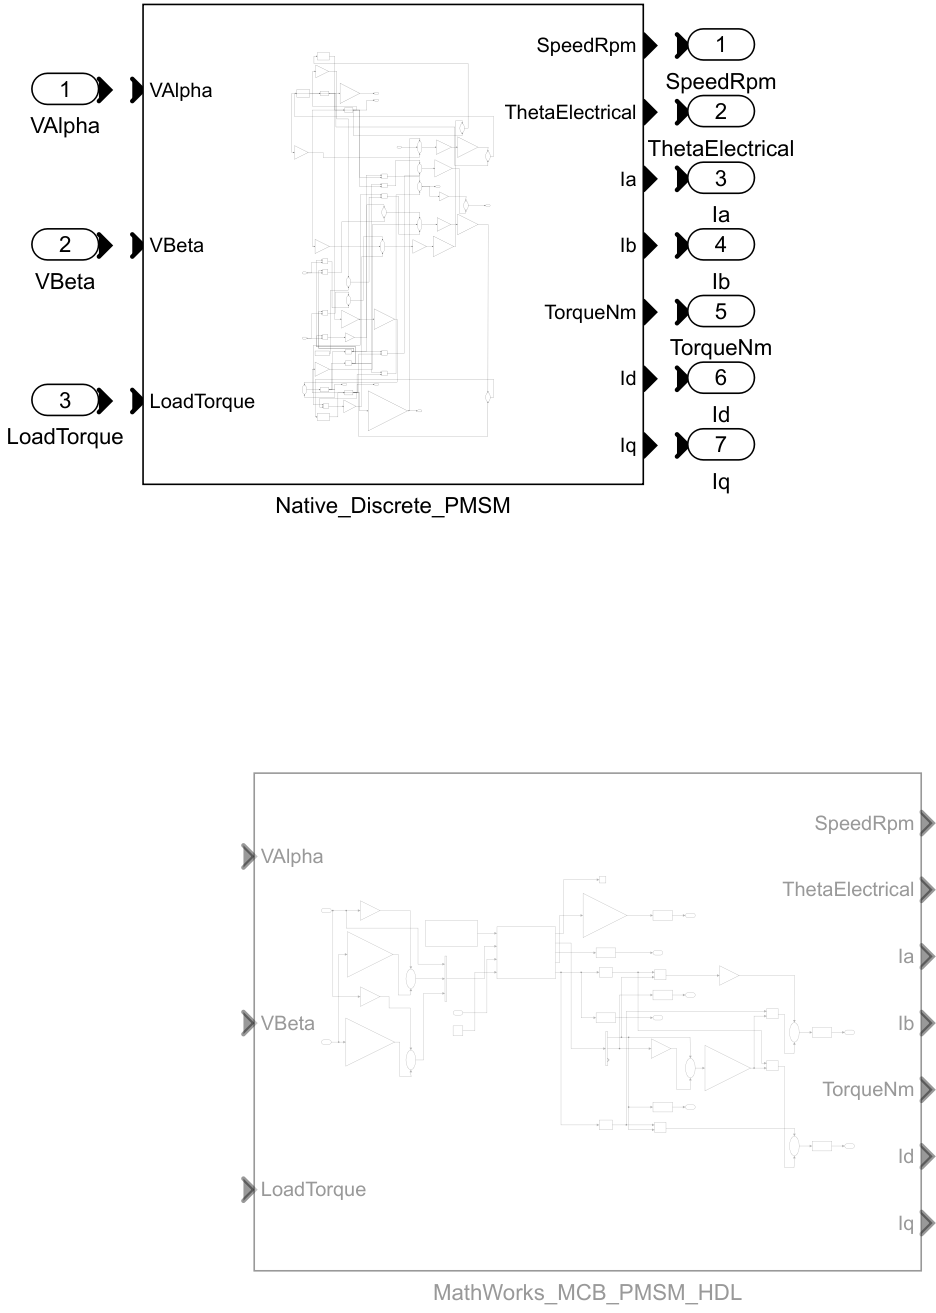
\includegraphics[width=0.98\textwidth]{PMSM_FOC_DualPlant_v21_plant_variants.png}
  \caption{Native 离散 PMSM 与 MathWorks PMSM HDL Variant 分支}
  \label{fig:plant-variants}
\end{figure}

\section{控制组件与任务边界}
\sectionline

速度环与电流环未混放。速度 PI 的离散状态每 1 ms 更新；显式 Rate Transition 将 $I_q^*$ 传到 $100\,\mu\mathrm{s}$ 任务；测量有效性、Clarke/Park、D/Q 电流 PI、解耦、限压/抗饱和、电压合成、逆变换、SVPWM、快速保护、故障锁存和最终 PWM 仲裁位于快速任务。命令优先级、Stateflow、过速/母线监测、诊断和状态发布位于 1 ms 任务。通信、参数维护、日志和非实时统计不进入控制器快环。

\begin{table}[H]
\centering
\caption{组件级任务调度、预算与数据合同}
\label{tab:tasks}
\scriptsize
\begin{tabularx}{0.98\textwidth}{p{0.12\textwidth}p{0.23\textwidth}p{0.13\textwidth}p{0.23\textwidth}X}
\toprule
\textbf{周期/相位} & \textbf{组件} & \textbf{WCET 预算} & \textbf{输入来源} & \textbf{输出消费者} \\
\midrule
$100\,\mu\mathrm{s}$/0 & 有效性、偏置校准、Clarke/Park/角度 & 14 $\mu$s & ADC/位置反馈、校准许可快照 & 电流 PI、快速保护、诊断 \\
$100\,\mu\mathrm{s}$/0 & d/q PI、解耦、限压/抗饱和、电压合成 & 24 $\mu$s & Id/Iq、IqRef 原子快照、参数 & 逆变换、状态诊断 \\
$100\,\mu\mathrm{s}$/0 & 逆变换与 SVPWM & 16 $\mu$s & Vd/Vq、角度、Vdc & 原始 DutyA/B/C 请求 \\
$100\,\mu\mathrm{s}$/0 & 快速保护、故障锁存、PWM 仲裁 & 16 $\mu$s & 电流/有效性、慢故障快照、监督请求、HardwareGate & PwmEnable、FaultBits/Code、执行器 \\
\textbf{$100\,\mu\mathrm{s}$ 合计} & \textbf{快任务} & \textbf{70 $\mu$s} & \multicolumn{2}{l}{预留 30 $\mu$s 调度/中断裕量} \\
1 ms/0 & 命令优先级、速度 PI、Stateflow & 220 $\mu$s & Start/Stop/Reset、速度、锁存故障快照 & IqRef、监督请求、模式控制 \\
1 ms/0 & 慢保护、诊断和状态发布 & 180 $\mu$s & 转速、Vdc、快任务状态快照 & 慢故障、状态 Bus \\
\textbf{1 ms 合计} & \textbf{慢任务} & \textbf{400 $\mu$s} & \multicolumn{2}{l}{预留 600 $\mu$s 集成裕量；通信/维护不进入快环} \\
\bottomrule
\end{tabularx}
\end{table}

上述 WCET 为设计分配预算，不是 Windows MIL 或最终 MCU 上的实测执行时间；目标硬件 WCET/PIL 仍属于 M9。所有跨速率量均经过命名 Rate Transition；慢到快的保护布尔量使用“保持数据完整性、关闭最大延迟确定性”的最小延迟配置，以满足 Stop 到最终 PWM 不超过 1 个慢环的合同。硬件门极关断目标为硬件立即生效；模型 \code{HardwareGate} 在当前快周期生效；软件过流/测量无效不超过 1 个快环；状态/启停不超过 1 个慢环。

\begin{landscape}
\thispagestyle{empty}
\begin{figure}[H]
  \centering
  
\includegraphics[width=0.98\linewidth]{PMSM_FOC_DualPlant_v21_controller_architecture.png}
  \caption{独立组件构成的 FOC 控制器及 Stateflow 门控结构}
  \label{fig:controller-architecture}
\end{figure}
\end{landscape}

{\footnotesize
\setlength{\tabcolsep}{3pt}
\begin{longtable}{>{\raggedright\arraybackslash}p{0.20\textwidth}
                  >{\raggedright\arraybackslash}p{0.25\textwidth}
                  >{\raggedright\arraybackslash}p{0.27\textwidth}
                  >{\raggedright\arraybackslash}p{0.20\textwidth}}
\caption{FOC 组件职责、接口与关键边界}\label{tab:foc-components}\\
\toprule
\textbf{组件} & \textbf{单一责任} & \textbf{主要接口} & \textbf{参数/约束} \\
\midrule
\endfirsthead
\multicolumn{4}{l}{\small 表 \thetable\ （续）}\\
\toprule
\textbf{组件} & \textbf{单一责任} & \textbf{主要接口} & \textbf{参数/约束} \\
\midrule
\endhead
\midrule
\multicolumn{4}{r}{\small 下页续}\\
\endfoot
\bottomrule
\endlastfoot

{\ttfamily\scriptsize Speed\_PI\_\allowbreak Controller\_1ms} &
速度误差变换为 $q$ 轴电流给定 &
\code{SpeedReferenceRpm}, \code{SpeedRpm} $\rightarrow$ \code{IqReference} &
1 ms；$K_p=0.02$，$K_i=0.05$；$\pm8$ A；非 RUN 清零积分器 \\

{\ttfamily\scriptsize Current\_Offset\_\allowbreak Calibration\_100us} &
对静止 A/B 相采样求均值并保持偏置，输出校正电流 &
Raw Ia/Ib、Enable/Reset $\rightarrow$ Corrected Ia/Ib、Offset、Done &
100 样本；$100\,\mu\mathrm{s}$；INIT/FAULT 清零 \\

{\ttfamily\scriptsize IqRef\_Rate\_\allowbreak Transition} &
确定性跨速率传递 $I_q^*$ &
1 ms \code{IqReference} $\rightarrow$ $100\,\mu\mathrm{s}$ 数据 &
显式 1 ms 到 $100\,\mu\mathrm{s}$ 边界 \\

\code{Clarke_Transform} &
$a/b$ 相电流转换到 $\alpha/\beta$ &
\code{Ia}, \code{Ib} $\rightarrow$ \code{Ialpha}, \code{Ibeta} &
$I_\alpha=I_a$；$I_\beta=(I_a+2I_b)/\sqrt{3}$ \\

{\ttfamily\scriptsize Electrical\_Angle\_\allowbreak Trig\_100us} &
集中计算一次电角度正弦和余弦并复用 &
$\theta_e$ $\rightarrow$ \code{SinTheta}, \code{CosTheta} &
$100\,\mu\mathrm{s}$；生成代码仅 1 次 \code{sinf} 和 1 次 \code{cosf} \\

\code{Park_Transform} &
$\alpha/\beta$ 电流转换到 $d/q$ &
\code{Ialpha}, \code{Ibeta}, Sin/Cos $\rightarrow$ \code{Id}, \code{Iq} &
与逆 Park 复用同一组角度三角函数 \\

\code{D_Axis_Current_PI} &
将 $I_d$ 调节到 0 A &
$I_d^*=0$, \code{Id} $\rightarrow$ \code{VdPI} &
$K_p=1$，$K_i=500$；积分限幅 $\pm30$ \\

\code{Q_Axis_Current_PI} &
跟踪速度环给出的 $I_q^*$ &
\code{IqReference}, \code{Iq} $\rightarrow$ \code{VqPI} &
$K_p=1$，$K_i=500$；积分限幅 $\pm30$ \\

{\ttfamily\scriptsize DQ\_Decoupling\_\allowbreak Feedforward} &
补偿交叉耦合和反电动势 &
Speed, \code{Id}, \code{Iq} $\rightarrow$ \code{VdFF}, \code{VqFF} &
极对数、$L_d$、$L_q$、$\lambda_{pm}$ \\

\code{DQ_Voltage_Command} &
叠加 PI 与前馈电压 &
PI/FF $\rightarrow$ \code{VdCommand}, \code{VqCommand} &
d/q 轴分别限幅 $\pm26$ V \\

{\ttfamily\scriptsize Alignment\_DQ\_\allowbreak Override\_100us} &
仅在 ALIGN 状态选择固定对齐命令 &
FOC Vd/Vq、反馈 Sin/Cos、AlignmentEnable $\rightarrow$ Applied Vd/Vq/Sin/Cos &
$V_d=2$ V，$V_q=0$ V，$\sin\theta=0$，$\cos\theta=1$ \\

{\ttfamily\scriptsize Inverse\_Park\_\allowbreak Transform} &
$d/q$ 电压转换到 $\alpha/\beta$ &
\code{Vd}, \code{Vq}, Applied Sin/Cos $\rightarrow$ \code{Valpha}, \code{Vbeta} &
$100\,\mu\mathrm{s}$ 快速链；不重复求三角函数 \\

{\ttfamily\scriptsize Inverse\_Clarke\_\allowbreak Transform} &
$\alpha/\beta$ 电压转换到三相 &
\code{Valpha}, \code{Vbeta} $\rightarrow$ \code{Va/Vb/Vc} &
B/C 相系数 $\pm\sqrt{3}/2$ \\

{\ttfamily\scriptsize SVPWM\_Duty\_Calculation} &
公共模注入并计算三相占空比 &
\code{Va/Vb/Vc}, \code{Vdc} $\rightarrow$ \code{DutyA/B/C} &
$V_{off}=-0.5(V_{max}+V_{min})$；0.02--0.98 \\
\end{longtable}
}

\section{数据字典与 Bus 接口契约}
\sectionline

\path{PMSM_FOC_Data.sldd} 是控制器设计数据的唯一来源。字典包含 30 个控制、保护、校准和数学参数，以及 41 个接口元素；旧 \code{PMSM_StartThreshold_Rpm} 已删除。参数目录逐项记录名称、目标类型、单位、范围、默认值、所有者、版本、数据类别和说明。参数集版本为 \code{2.1.0}，兼容性标识为 \code{PMSM_FOC_DUALPLANT_V21}。CRC 字段明确保留给后续标定导出流水线，不作为当前构建的虚假校验值。

\begin{table}[H]
\centering
\caption{设计数据分类与代码属性}
\label{tab:data-classes}
\small
\begin{tabularx}{0.95\textwidth}{p{0.23\textwidth}p{0.25\textwidth}X}
\toprule
\textbf{类别} & \textbf{典型对象} & \textbf{约束与用途} \\
\midrule
CompileTimeConstant & 任务周期、数学系数、安全占空比 & 作为算法/调度不变量，允许代码生成器内联 \\
TunableCalibration & PI、限幅、保护阈值、校准/对齐参数 & \code{Simulink.Parameter}，生成可识别的标定全局量 \\
RuntimeSignal & 命令、测量及跨任务数据 & 由类型化 Bus 交换，并在接口目录记录更新周期 \\
ReadOnlyDiagnostic & Duty、状态码、故障码、限幅状态 & 仅由控制器写入 \code{ControlStatusBus}，上层不得反向修改 \\
\bottomrule
\end{tabularx}
\end{table}

\begin{table}[H]
\centering
\caption{控制器 Bus 契约摘要}
\label{tab:bus-contracts}
\small
\begin{tabularx}{0.97\textwidth}{p{0.20\textwidth}p{0.47\textwidth}X}
\toprule
\textbf{Bus} & \textbf{元素} & \textbf{责任边界} \\
\midrule
\code{ControlCommandBus} & Start/Stop/EmergencyStop、DriverFault、HardwareGate、Direction、Speed/Torque Reference、FaultResetRequest & 显式命令与硬件许可；优先级为故障/急停 $>$ Stop $>$ Start \\
\code{MeasurementBus} & Ia/Ib/Ic、Vdc、电角度、机械速度、Valid、Timestamp、Freshness & Valid 已进入快速禁止；Timestamp/Freshness 留给 MEAS-001 \\
\code{ControlStatusBus} & 原始 Duty 请求、Id/Iq、Vd/Vq、最终 PwmEnable、StateCode、FaultBits/Code、限幅和测量状态 & Duty 必须与 PwmEnable 配套使用；状态经 Rate Transition 发布 \\
\code{CalibrationBus} & 电流偏置、对齐电压/时间、样本数、版本、CRC & 字典中的等价标定结构，避免顶层参数散线 \\
\bottomrule
\end{tabularx}
\end{table}

控制器根端口由 7 入/8 出标量改为 \code{2BI-1BO}。生成代码输出 \code{ControlCommandBus.h}、\code{MeasurementBus.h} 和 \code{ControlStatusBus.h}；\code{ExtU/ExtY} 与模型端口使用同名类型。

Duty 和 PwmEnable 按 100 $\mu$s 发布，状态码与 $I_q^*$ 每 1 ms 更新。两个状态发布 Rate Transition 保持慢任务最近原子快照，不增加慢组件执行频率。

\code{FaultBits/FaultCode} 由 100 $\mu$s 故障锁存管理器直接输出；\code{CurrentLimitActive} 对应软件过流锁存位；\code{VoltageLimitActive} 仍为 false，占位语义由 CTL-001/002 后续替换。

\section{Stateflow 电机状态管理}
\sectionline

\code{Motor_Supervisor_1ms} 是运行模式和 \code{SupervisorPwmRequest} 的所有者，不直接拥有最终 PWM 许可。顶层 \code{SUPERVISED} 父状态包含 INIT、READY、CALIB、ALIGN 和 RUN，并以统一故障迁移进入顶层 FAULT。Chart 输入为 \code{StartAccepted}、\code{StopActive}、\code{FaultDetected}、\code{ResetAllowed} 和 \code{CalibrationDone}；数值平均、电压选择、故障锁存和最终仲裁由独立 Simulink 组件负责。

\begin{figure}[H]
  \centering
  \begin{tikzpicture}[
    >=Stealth,
    node distance=7mm and 7mm,
    st/.style={draw=navy,rounded corners=2pt,fill=lightblue,
      minimum width=25mm,minimum height=13mm,align=center,font=\small},
    fault/.style={draw=red!70!black,rounded corners=2pt,fill=red!10,
      minimum width=30mm,minimum height=13mm,align=center,font=\small},
    flow/.style={->,thick,draw=navy,font=\scriptsize}]
    \node[st] (init) {INIT\\复位状态};
    \node[st,right=of init] (ready) {READY\\等待启动};
    \node[st,right=of ready] (calib) {CALIB\\100 样本校准};
    \node[st,right=of calib] (align) {ALIGN\\2 V d 轴对齐};
    \node[st,right=of align] (run) {RUN\\闭环 FOC};
    \node[fault,below=16mm of calib] (fault) {FAULT\\PWM 关闭并锁存};
    \node[draw=blue,dashed,rounded corners=3pt,fit=(init)(ready)(calib)(align)(run),
      inner sep=4mm,label={[font=\scriptsize,blue]above:SUPERVISED}] (super) {};
    \draw[flow] (init) -- node[above]{1 tick} (ready);
    \draw[flow] (ready) -- node[above]{StartAccepted} (calib);
    \draw[flow] (calib) -- node[above]{Done} (align);
    \draw[flow] (align) -- node[above]{20 tick} (run);
    \draw[flow] (super.south) -- node[right]{任一故障/校准超时} (fault.north);
    \draw[flow] (fault.west) to[bend left=22]
      node[left,align=right]{ResetAllowed\\且故障消失} (init.south);
    \node[font=\scriptsize,text=navy,anchor=north east,align=right]
      at (super.south east) {CALIB/ALIGN/RUN：StopActive $\Rightarrow$ INIT};
  \end{tikzpicture}
  \caption{1 ms Stateflow 顶层状态、职责和锁存故障路径（LaTeX 重绘）}
  \label{fig:stateflow-architecture}
\end{figure}

\begin{table}[H]
\centering
\caption{Stateflow 状态定义与输出}
\label{tab:states}
\footnotesize
\begin{tabularx}{0.95\textwidth}{p{0.10\textwidth}p{0.15\textwidth}XXp{0.12\textwidth}}
\toprule
\textbf{代码} & \textbf{状态} & \textbf{职责} & \textbf{退出条件} & \textbf{控制/请求} \\
\midrule
1 & INIT & 清空校准状态和速度/电流 PI & 1 个 tick 后进入 READY & 控制 0 / 请求 0 \\
2 & READY & 保持 PI 复位，等待有效启动命令 & \code{StartAccepted} 且非 Stop 后进入 CALIB & 控制 0 / 请求 0 \\
3 & CALIB & 使能字典配置样本数的电流偏置平均 & \code{CalibrationDone} 进入 ALIGN；\code{PMSM_Calibration_}\newline\code{TimeoutTicks} 超时进 FAULT & 控制 0 / 请求 0 \\
4 & ALIGN & 施加字典配置的 d/q 电压和固定角度 & \code{PMSM_Alignment_}\newline\code{DurationTicks} 后进入 RUN；停止回 INIT & 控制 0 / 请求 1 \\
5 & RUN & 放行速度给定和闭环 SVPWM & 停止回 INIT；任一故障进 FAULT & 控制 1 / 请求 1 \\
6 & FAULT & 撤销 PWM 请求、清空 PI/校准并保持锁存 & FaultResetRequest、故障消失且停止后回 INIT & 控制 0 / 请求 0 \\
\bottomrule
\end{tabularx}
\end{table}

状态机以 1 ms tick 执行，正常启动序列为 INIT $\rightarrow$ READY $\rightarrow$ CALIB $\rightarrow$ ALIGN（20 ms）$\rightarrow$ RUN；校准数值组件仍以 $100\,\mu\mathrm{s}$ 累积 100 个样本。测试速度命令在 0.05 s 上升，0.06 s 完成校准，模型于 0.08 s 进入 RUN。

\subsection{安全监测与输出门控}

\code{Fast_Protection_100us} 只产生软件过流和测量无效原始条件；\code{Slow_Safety_Monitor_1ms} 保留过速、欠压、过压的独立身份；\code{Fault_Latch_Manager_100us} 是故障位、主码、锁存和复位的唯一所有者。\code{Final_PWM_Arbiter_100us} 是唯一最终关断点：

\begin{center}
\fcolorbox{navy}{lightblue}{\ttfamily FinalPwmEnable = SupervisorPwmRequest \&\& FastInterlock \&\& HardwareGate}
\end{center}

任一输入都能独立在 100 $\mu$s 任务中撤销许可。故障位 0--6 依次为 EmergencyStop、DriverFault、软件过流、测量无效、过速、欠压和过压；主码为相应的 1--7，数字较小者优先。复位只有在 Stop 有效、Start 清除、HardwareGate 为真且全部原始故障消失时允许。控制器 Duty 不因关断改为 0.5；Harness 平均值对象内部的 \code{Average_Plant_Enable_Map} 才把禁用映射为三相相等占空比以获得零线电压。

\begin{table}[H]
\centering
\caption{故障判据与安全动作}
\label{tab:safety}
\footnotesize
\begin{tabularx}{0.94\textwidth}{p{0.18\textwidth}p{0.22\textwidth}p{0.20\textwidth}X}
\toprule
\textbf{监测项} & \textbf{触发阈值} & \textbf{任务所有者} & \textbf{安全动作} \\
\midrule
EmergencyStop & 外部布尔电平 & $100\,\mu\mathrm{s}$ 锁存管理器 & 位 0/码 1；当前快周期关断并锁存 \\
DriverFault & 驱动器布尔故障 & $100\,\mu\mathrm{s}$ 锁存管理器 & 位 1/码 2；当前快周期关断并锁存 \\
A/B 相电流 & \code{PMSM_Protection_}\newline\code{MaxCurrent_A}（默认 12 A） & $100\,\mu\mathrm{s}$ 快速保护 & 位 2/码 3；不超过 1 个快环 \\
Measurement.Valid & false & $100\,\mu\mathrm{s}$ 快速保护 & 位 3/码 4；当前快周期关断并锁存 \\
机械转速 & \code{PMSM_Protection_}\newline\code{MaxSpeed_Rpm}（默认 3000 rpm） & 1 ms 慢保护 & 位 4/码 5；经快照进入锁存管理器 \\
直流母线 & \code{PMSM_Protection_}\newline\code{MinDcBus_V / MaxDcBus_V}（默认 10/60 V） & 1 ms 慢保护 & 欠压位 5/码 6；过压位 6/码 7 \\
\bottomrule
\end{tabularx}
\end{table}

\section{被控对象与关键参数}
\sectionline

两个 Variant 分支具有一致的 3 输入/7 输出接口：输入为 \code{VAlpha}、\code{VBeta} 和 \code{LoadTorque}；输出为 \code{SpeedRpm}、\code{ThetaElectrical}、\code{Ia}、\code{Ib}、\code{TorqueNm}、\code{Id} 和 \code{Iq}。默认选择值为 2，即 MathWorks \code{mcbhdlplantlib/PMSM HDL} 分支。

\begin{table}[H]
\centering
\caption{仿真工况及电机参数}
\label{tab:parameters}
\small
\begin{tabularx}{0.94\textwidth}{p{0.15\textwidth}p{0.43\textwidth}X}
\toprule
\textbf{类别} & \textbf{参数} & \textbf{数值} \\
\midrule
工况 & 速度给定 & 0.05 s 时由 0 阶跃至 1000 rpm \\
工况 & 负载转矩 & 0.5 s 时由 0 阶跃至 0.2 N$\cdot$m \\
仿真 & 求解器、步长、时长 & FixedStepDiscrete，$100\,\mu\mathrm{s}$，2.0 s \\
电源 & 直流母线电压 & 48 V \\
电机 & 定子电阻 $R_s$ & 0.4 $\Omega$ \\
电机 & $L_d$、$L_q$ & 1 mH、1 mH \\
电机 & 永磁磁链 $\lambda_{pm}$ & 0.05 Wb \\
电机 & 极对数 & 4 \\
电机 & 转动惯量 $J$ & 0.002 kg$\cdot$m$^2$ \\
电机 & 黏性阻尼 $B$ & 0.0001 N$\cdot$m$\cdot$s/rad \\
\bottomrule
\end{tabularx}
\end{table}

\section{自动测试与结果}
\sectionline

构建脚本执行 Native 与 MathWorks 两个 2 s 闭环场景、正常启动、已知偏置校准、ALIGN 电压输出、慢/快速保护、故障锁存、确认复位、组件/连线/速率结构检查以及控制器 ERT 代码生成。专项脚本 \code{verify_pmsm_foc_command_safety_v21} 进一步覆盖无 Start、命令冲突、急停、驱动故障、测量无效、HardwareGate、Stop 延迟、故障位码、复位条件和单点仲裁。所有测试使用 MATLAB/Simulink/Stateflow R2024a。

\begin{figure}[H]
  \centering
  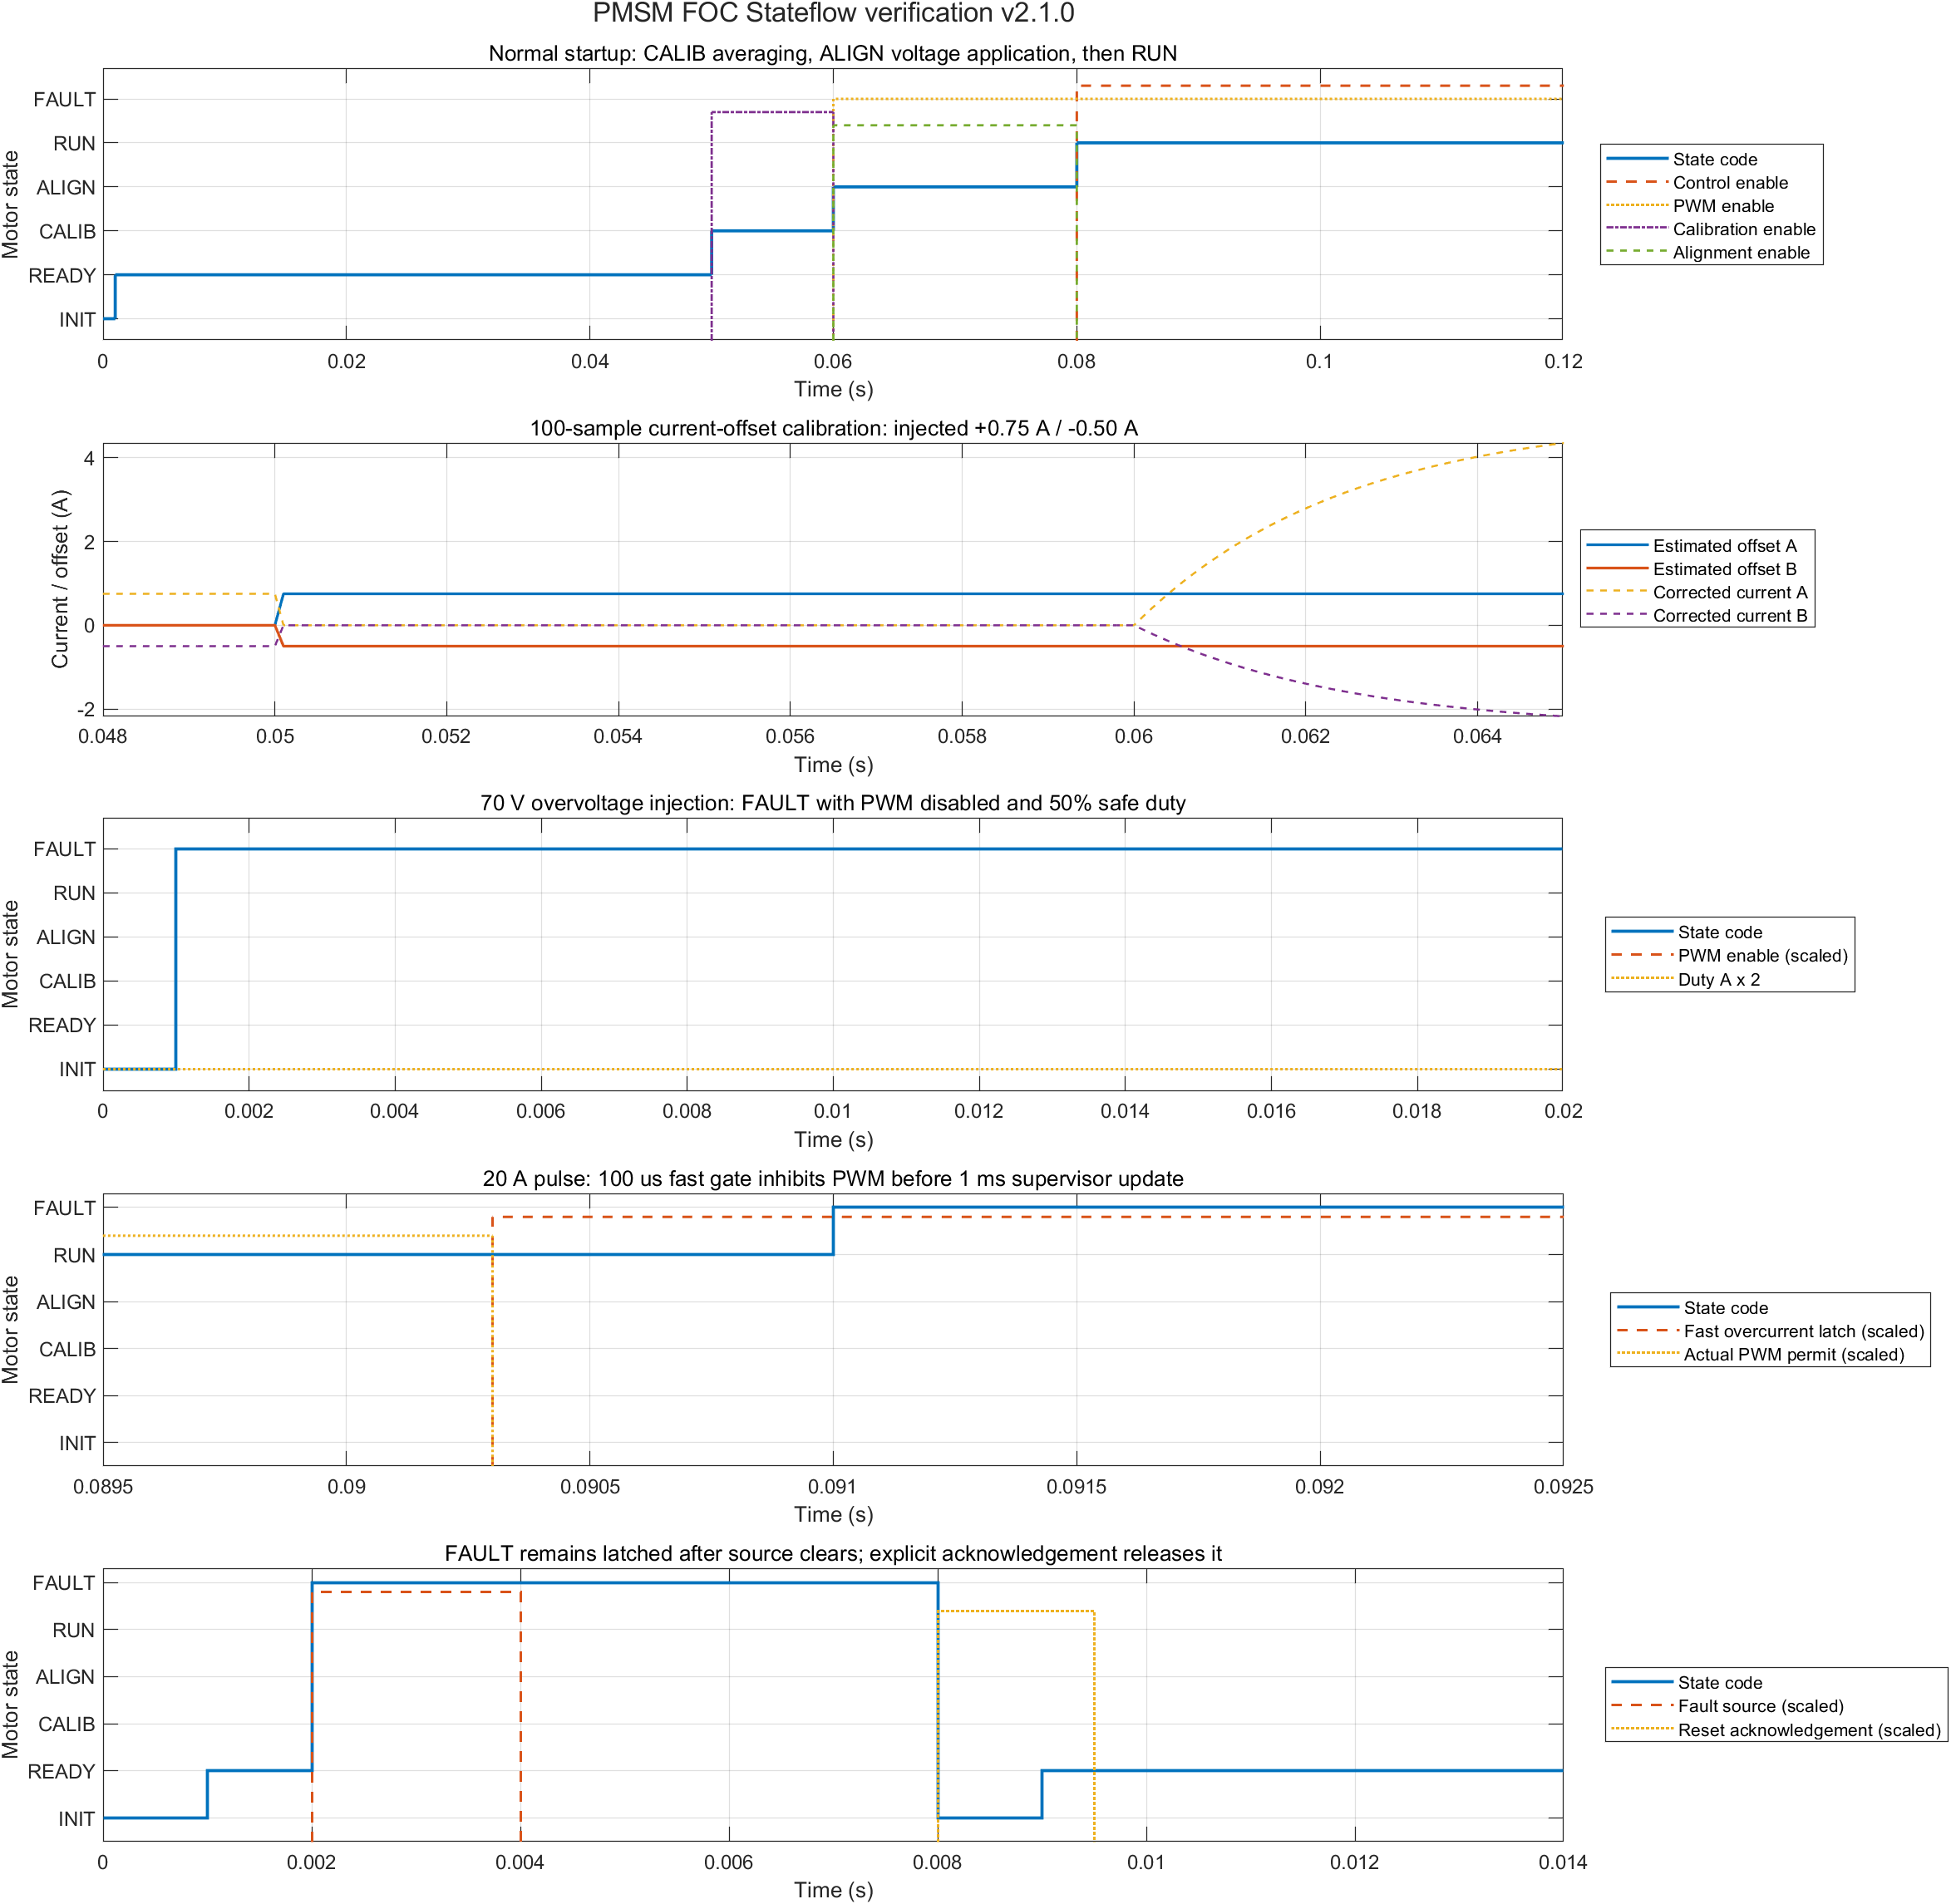
\includegraphics[width=0.98\textwidth]{PMSM_FOC_DualPlant_v21_stateflow_results.png}
  \caption{Stateflow 启动、校准、对齐、慢速过压、快速过流和确认复位结果}
  \label{fig:stateflow-results}
\end{figure}

\begin{figure}[H]
  \centering
  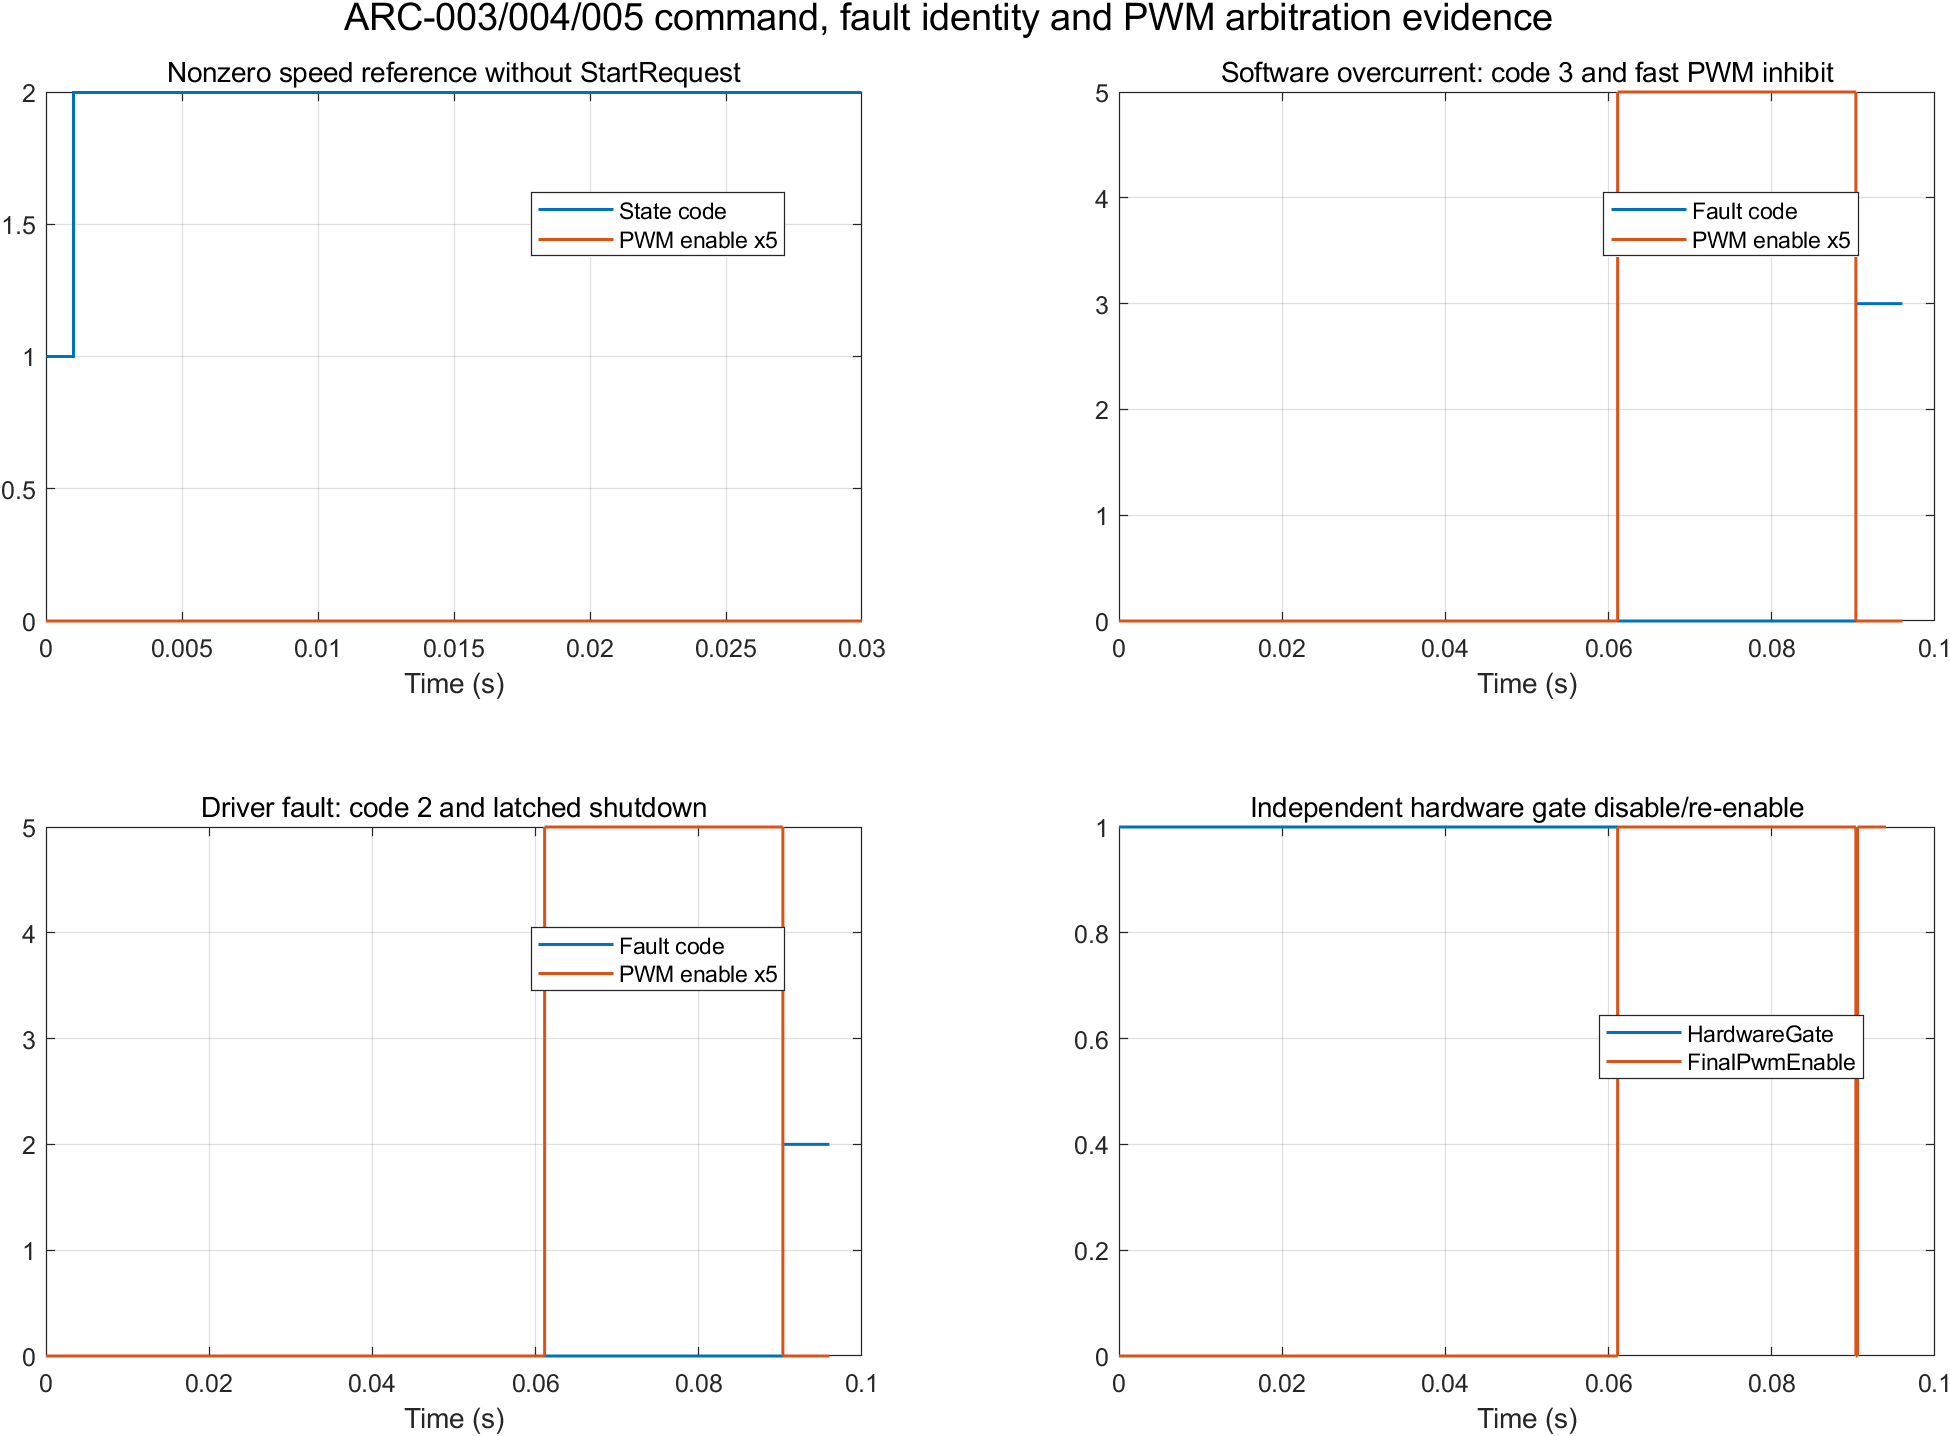
\includegraphics[width=0.98\textwidth]{arc003_arc005_command_safety_test.png}
  \caption{ARC-003--005 无启动、过流、驱动故障和 HardwareGate 专项证据}
  \label{fig:arc003-005-results}
\end{figure}

\begin{table}[H]
\centering
\caption{Stateflow 测试验收结果}
\label{tab:stateflow-tests}
\small
\begin{tabularx}{0.95\textwidth}{p{0.28\textwidth}Xp{0.13\textwidth}}
\toprule
\textbf{测试} & \textbf{观察结果} & \textbf{结论} \\
\midrule
正常启动与对齐 & 访问 [1 2 3 4 5]；0.08 s 进入 RUN；ALIGN 时 AppliedVd=2 V、AppliedVq=0 V 且 PWM 有效 & \pass \\
电流偏置校准 & 注入 $+0.75/-0.50$ A；0.06 s 估计为 $+0.75/-0.50$ A；完成时校正电流均为 0 A & \pass \\
70 V 过压注入 & 访问 [1 6]；1 ms 慢保护在 0.001 s 进入 FAULT；DutyA=0.5 & \pass \\
20 A 快速过流 & 0.0903 s 注入持续 0.2 ms 的脉冲；同一时间快速故障和 PWM 禁止生效，测得延迟 0 $\mu$s & \pass \\
非零速度给定但无 Start & 只访问 INIT/READY，最终和全程 PwmEnable 均为 0 & \pass \\
Start/Stop 冲突与 Stop 延迟 & 同时有效时 Stop 获胜；RUN 中 Stop 到 INIT 为 0.7 ms & \pass \\
EmergencyStop / DriverFault & PwmEnable 关断延迟均为 0 $\mu$s；位码分别为 1/1、2/2 & \pass \\
测量无效 & Valid=false 同周期关断；FaultBits/FaultCode=8/4 & \pass \\
HardwareGate & 独立同周期关断和恢复，FaultBits 保持 0 & \pass \\
任意状态故障锁存 & 分别从 INIT/READY/CALIB/ALIGN/RUN 注入短脉冲；故障源清除后五项均保持 FAULT & \pass \\
确认复位 & 只有 Stop、Start 清除、HardwareGate、原始故障全清和 FaultResetRequest 同时满足才退出 & \pass \\
状态/速率/代码结构 & 6 状态、唯一 PWM 仲裁、17 个 Rate Transition、2BI-1BO；30 参数/41 接口；ERT 检查通过 & \pass \\
\bottomrule
\end{tabularx}
\end{table}

\begin{figure}[H]
  \centering
  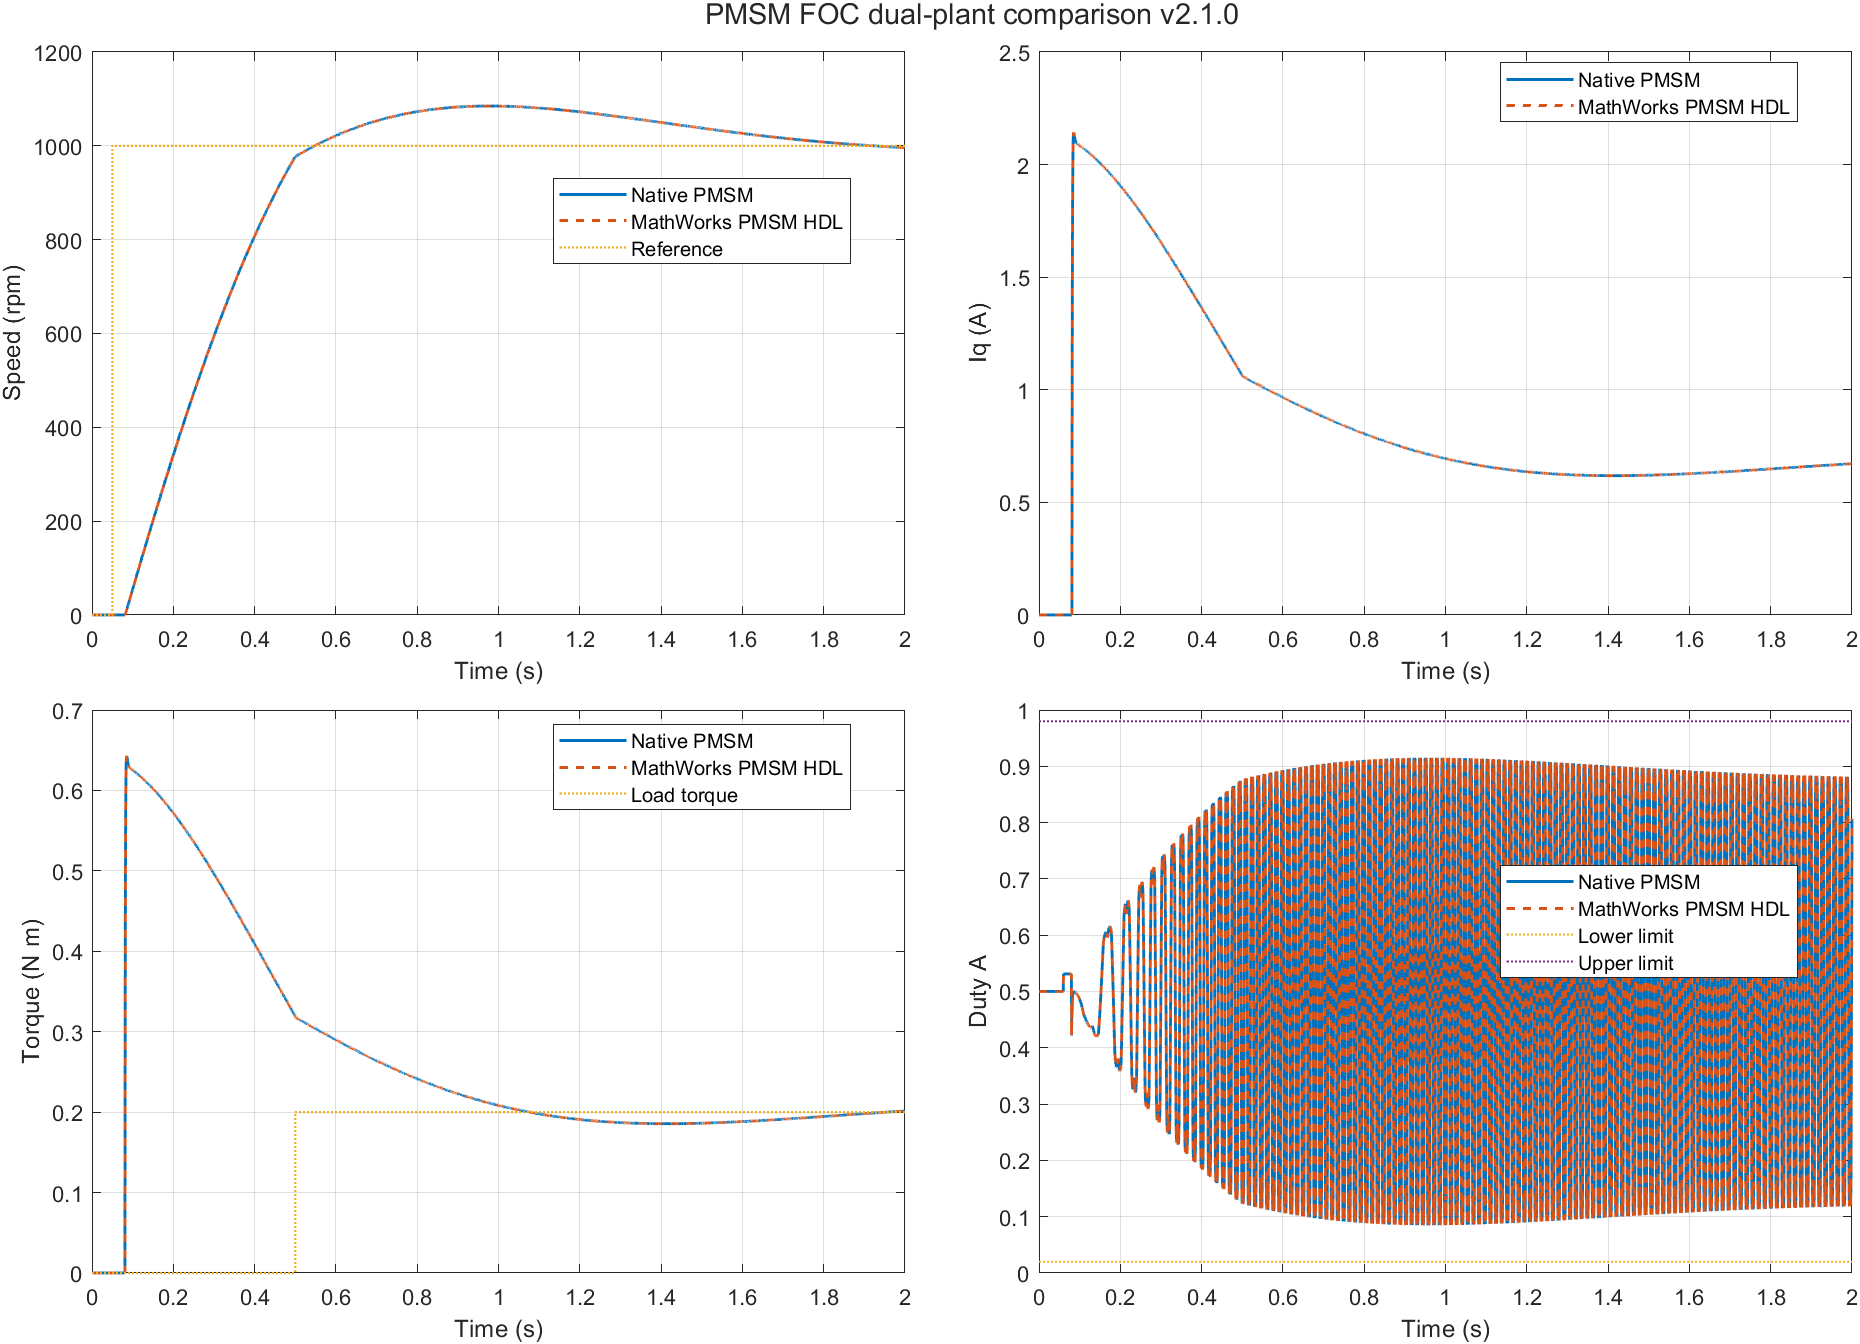
\includegraphics[width=0.98\textwidth]{PMSM_FOC_DualPlant_v21_results.png}
  \caption{两个 PMSM 被控对象的速度、$I_q$、转矩和 Duty A 曲线}
  \label{fig:plant-results}
\end{figure}

\begin{table}[H]
\centering
\caption{双被控对象闭环验收结果}
\label{tab:plant-tests}
\small
\begin{tabularx}{0.94\textwidth}{X>{\raggedleft\arraybackslash}p{0.27\textwidth}>{\raggedleft\arraybackslash}p{0.27\textwidth}}
\toprule
\textbf{指标} & \textbf{Native 离散 PMSM} & \textbf{MathWorks PMSM HDL} \\
\midrule
最终转速 & 996.191467 rpm & 996.191345 rpm \\
最大转速 & 1084.86560 rpm & 1084.86560 rpm \\
最大绝对 $I_q$ & 2.14349961 A & 2.14349937 A \\
Duty A 最小值 & 0.0849514306 & 0.0849514306 \\
Duty A 最大值 & 0.915057063 & 0.915057063 \\
最终电磁转矩 & 0.201538101 N$\cdot$m & 0.201538414 N$\cdot$m \\
闭环限值检查 & \pass & \pass \\
\bottomrule
\end{tabularx}
\end{table}

结构及代码检查还确认：
\begin{itemize}[nosep,leftmargin=2em]
  \item Variant 分支数为 2，显式命令、FOC、快/慢保护、锁存和仲裁组件均存在；
  \item 控制器接口为 2 个 Bus 输入/1 个 Bus 输出，旧 \code{FaultResetAck} 标量端口不存在；
  \item 数据字典含 30 个参数和 41 个接口元素，旧隐式启动参数不存在，四类 Bus 逐元素检查通过；
  \item 速度、Stateflow 和慢保护任务均为 0.001 s；电流与快速安全门任务均为 0.0001 s；
  \item 17 个命名 Rate Transition、双速率调度器和快/慢安全逻辑均通过结构检查；
  \item 控制器与闭环模型悬空线数均为 0；
  \item 生成代码包含三个 Bus 头文件、\code{DriverFault}、\code{HardwareGate}、\code{FaultBits}、最终 \code{PwmEnable} 和 Stateflow 逻辑；旧 StartThreshold 与 S-Function 文本不存在，综合结论为 \pass。
\end{itemize}

\subsection{BASE-002 需求追溯与架构符合性}

原始架构 M0--M10 已拆分为 22 条唯一需求。完整矩阵位于 \path{doc/PMSM_FOC_v2.1.0_Requirements_Traceability_Matrix.md}，每行均包含需求来源、状态、模型/数据路径、生成代码符号、测试证据、设计偏离和风险。状态只允许“已满足、部分满足、未满足、明确延期”，因此未实现的观察器、无传感器切换和硬件验证不会被当前 MIL/代码生成结果掩盖。

\begin{table}[H]
\centering
\caption{M0--M10 需求状态汇总}
\label{tab:traceability-summary}
\small
\begin{tabularx}{0.94\textwidth}{p{0.20\textwidth}p{0.13\textwidth}X}
\toprule
\textbf{状态} & \textbf{数量} & \textbf{代表性范围} \\
\midrule
已满足 & 10 & M0 数据字典/Bus、M1 PI、M2 可切换对象、M3 FOC/双速率、M4 聚合有效性、M6 状态机/故障、M9 ERT 代码生成 \\
部分满足 & 5 & M1 对象级阶跃、M2 dq 对象验收、M5 编码器/工况、M9 SIL/PIL/实时集成 \\
未满足 & 1 & M4 双电阻窗口、重构、死区和不可测区降级 \\
明确延期 & 6 & M7 观察器、M8 无传感器切换、M10 低压/目标电压硬件验证 \\
\bottomrule
\end{tabularx}
\end{table}

主要剩余偏离包括：Direction/TorqueReference 尚未形成运行模式；故障历史/冻结帧未实现；\code{FreshnessTicks} 尚未形成超时策略；电压矢量限幅诊断、SIL/PIL、真实 MCU WCET 和硬件关断链仍待闭环；CRC 是受控占位符。显式启停、稳定故障位码、聚合 Valid 快速关断和双速率任务合同已由 ARC-003--005 完成。

\subsection{BASE-001 可复现基线}

ARC-003--005 之前曾在 2026 年 8 月 31 日使用 \code{verify_pmsm_foc_reproducibility_v21} 连续执行两次 clean build，结果如下表。它证明重建机制有效，但其 checksum 已因本轮显式命令、安全仲裁和速率边界变更而归档；本轮提交后必须重新运行才能形成新的发布基线。

\begin{table}[H]
\centering
\caption{可复现构建环境与配置清单}
\label{tab:repro-environment}
\small
\begin{tabularx}{0.96\textwidth}{p{0.30\textwidth}X}
\toprule
\textbf{项目} & \textbf{冻结值} \\
\midrule
主机环境 & Windows 11 专业版，win64 \\
MATLAB & R2024a，24.1.0.2537033 \\
必要产品 & MATLAB、Simulink、Stateflow、Simulink Coder、Embedded Coder、Motor Control Blockset，版本均为 24.1，许可检查均通过 \\
控制器求解器/步长 & Fixed-step / FixedStepDiscrete，0.0001 s \\
Harness 求解器/步长 & Fixed-step / FixedStepDiscrete，0.0001 s \\
控制器代码目标 & \code{ert.tlc}，Nonreusable function，Windows x86-64，自动工具链 \\
Harness 仿真目标 & \code{grt.tlc}，Nonreusable function，Windows x86-64 \\
构建 Git 基点 & \code{ae62bac49051591a13a38ac546a6ef5f7779cf93} \\
\bottomrule
\end{tabularx}
\end{table}

\begin{table}[H]
\centering
\caption{两次完全清理重建的一致性结果}
\label{tab:repro-results}
\small
\begin{tabularx}{0.96\textwidth}{p{0.34\textwidth}XX}
\toprule
\textbf{证据} & \textbf{第 1 轮} & \textbf{第 2 轮} \\
\midrule
构建耗时 & 444.868618 s（冷启动） & 46.7441007 s（热缓存） \\
控制器语义 checksum & \multicolumn{2}{l}{\code{F3830E96A301CAE4DD5FADBB6B09AFD8}，一致} \\
Harness 语义 checksum & \multicolumn{2}{l}{\code{5D7F7808CAEFDB7F3253245556780ACB}，一致} \\
接口签名 & \code{2BI-1BO-13C-6S} & \code{2BI-1BO-13C-6S} \\
Native 指标最大差值 & \multicolumn{2}{l}{0（容差 $1\times10^{-6}$）} \\
MCB 指标最大差值 & \multicolumn{2}{l}{0（容差 $1\times10^{-6}$）} \\
完整验证门禁 & \pass & \pass \\
\bottomrule
\end{tabularx}
\end{table}

表 \ref{tab:repro-results} 是 ARC-003--005 变更前的已归档 BASE-001 证据；本轮模型结构和 checksum 必然变化，不能再把旧 checksum 当作当前发布基线。当前命令/安全/速率/ERT 专项门禁已通过；正式发布前仍须在本轮提交后重新执行双轮 clean build，在 Git clean 状态刷新两个 checksum，并在第二台同配置开发机复跑。

\section{重建、切换与维护}
\sectionline

在 MATLAB 中将当前目录切换至 v2.1.0 模型目录并运行：

\begin{center}
\fcolorbox{navy}{lightgray}{\parbox{0.82\textwidth}{\ttfamily\centering build\_pmsm\_foc\_dualplant\_v21}}
\end{center}

脚本会创建/更新数据字典，重建组件和 Stateflow 集成，应用 Bus 根接口，依次仿真两个 Variant，执行校准、对齐、慢/快速保护、故障锁存和确认复位测试，验证连线、任务周期、参数影子和四类接口契约，生成控制器 ERT C 代码并更新 \path{verification_report.txt}。ARC-003--005 专项复核使用 \code{verify_pmsm_foc_command_safety_v21}，它更新 \path{arc003_arc005_verification_report.txt} 和测试曲线。集成脚本每次先恢复确定性的标量内部实现，因此不会积累红色虚线或重复连线；Harness 测试日志和平均值对象适配器不进入 ERT 控制器。

完全清理重建使用：

\begin{center}
\fcolorbox{navy}{lightgray}{\parbox{0.92\textwidth}{\ttfamily\centering build\_pmsm\_foc\_dualplant\_v21('CleanBuild', true, 'BatchMode', true, 'ExportImages', false)}}
\end{center}

冻结基线或发布前复核使用 \code{verify_pmsm_foc_reproducibility_v21}。该脚本仅在两轮 clean build 的模型语义校验和、接口、配置、关键指标及全部 PASS 门禁一致时返回成功。详细结果写入 \path{baseline_reproducibility_report.txt}。

\clearpage
\subsection*{模型切换}
模型工作区变量 \code{PMSM_PLANT_SELECTION} 控制被控对象：1 为 Native 离散 PMSM，2 为 MathWorks PMSM HDL（默认）。仿真停止时也可使用顶层 Dashboard 按钮切换，下一次仿真编译所选分支。

\section{结论}
\sectionline

v2.1.0 已明确职责边界：1 ms 命令仲裁和 Stateflow 管理模式与监督请求；1 ms 慢保护负责过速及母线电压；$100\,\mu\mathrm{s}$ 快速保护、故障锁存和唯一仲裁器分别拥有判定、记忆和最终 PWM 权限；独立组件执行偏置校准、对齐和数值 FOC。30 个设计参数、41 个接口元素、\code{2BI-1BO} 根接口和 M0--M10 的 22 条追溯需求已纳入手册。无 Start、Stop 优先级、0.7 ms Stop 状态响应、四类 0 $\mu$s 快速禁止、稳定故障位码、HardwareGate 独立关断/恢复、确认复位、17 个 Rate Transition、Bus C 类型和 ERT 代码生成均通过自动验收。真实硬件立即关断、目标 WCET/SIL/PIL、两电阻采样、观察器和硬件部署仍按追溯矩阵延期。

\end{document}
